%!TEX root = ../../PhD_thesis__Edouard_Leurent.tex

\graphicspath{{2-Chapters/1-Chapter/}}

\chapter{Introduction}
\label{chapter:1}

\begin{flushright}
	\begin{tabular}{@{}l@{}}
		\emph{Pour soulever un poids si lourd,}\\
		\emph{Sisyphe, il faudrait ton courage !}\\
		\emph{Bien qu’on ait du cœur à l’ouvrage,}\\
		\emph{L’Art est long et le Temps est court.}\\
	\end{tabular}

	Charles Baudelaire, \href{https://eleurent.github.io/sisyphe/texts/le-guignon.html}{\emph{Le guignon}}.
\end{flushright}

\section{Context and scope}


\paragraph{How should a driving robot make decisions?}

In the first few weeks of my PhD, I observed that layman interlocutors, when confronted to this question on the occasion of a social dinner, have a general tendency to conjure up disaster scenarios involving imminent accidents with unavoidable casualties. This reflex is likely to stem from the popularisation of the Trolley Problem \citep{Foot1967}, a famous thought experiment in Moral Philosophy, depicted in \Cref{fig:trolley}, in which a runaway trolley is headed straight toward five people tied up on the main track and unable to move. A lever, when pulled, switches the trolley to a side track occupied by one person: what should you do? Answering this general question of what we \emph{ought} to do in any situation, what is a \emph{right} or \emph{wrong} decision, is the focus of the field of {normative ethics}. This dilemma illustrates a clash between two schools of thought: utilitarianism and deontological ethics. According to utilitarians, the rightfulness of an action should be evaluated based on its consequences, and actions maximising a \emph{utility} --the happiness and well-being for the affected individuals-- should be preferred. Conversely, deontologists evaluate the morality of actions \emph{per se}, according to a series of rules, rather than based on their consequences. Although this problem was initially introduced as a thought experiment, its transposition to the context of autonomous driving and arguably more realistic scenarios made it heavily cited in discussions regarding safety \citep[e.g.][]{Lin2015,Bonnefon2016,Gogoll2017}. In early 2017, MIT’s Media Lab launched the \emph{Moral Machine} platform \citep{Awad2018}, in which members of the public were invited to select the morally acceptable decision out of several options available to an autonomous vehicle. The authors argued that the recovered global preference would provide \emph{"essential topics to be considered by policymakers"}, and \citep{Noothigattu2018} proposed an implementation of a system aggregating these preferences, trained on the collected data. However, the relevance of this analogy to inform engineering and policy has been called into question. Thus, \citep{DeFreitas2019} point out that such dilemma are unlikely to occur on real roads, hard to detect by perception systems and to act upon by control systems, and that they are distracting researchers from the more appropriate goal of how to avoid accidents altogether. Indeed, when we drive we seldom find ourselves in such extreme situations but rather constantly ponder over less tragic questions-- where does this vehicle intend to go? do I have the time to proceed? what is the appropriate speed to drive at right now? Thus, artificially reproducing this cognitive process of driving while avoiding accidents is more of a technical problem than an ethical one, and will constitute the object of this thesis. Yet, it would be illusory to pretend that the practical implications of the Trolley Problem cannot simply be swept aside and replaced by technicality: we will see that ethical concerns still underpin most assumptions and design choices of safety-critical software.

\begin{figure}[tp]
	\centering
	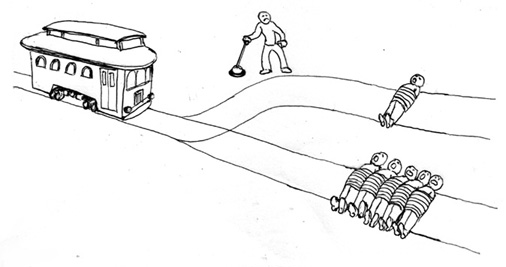
\includegraphics[width=0.7\linewidth]{img/trolley}
	\caption{The Trolley Problem \citep{Foot1967}. Illustration by \href{http://subcortex.com/}{Jesse J. Prinz}.}
	\label{fig:trolley}
\end{figure}

\paragraph{Nuts and bolts of self-driving software}

\begin{figure}[tp]
	\centering
	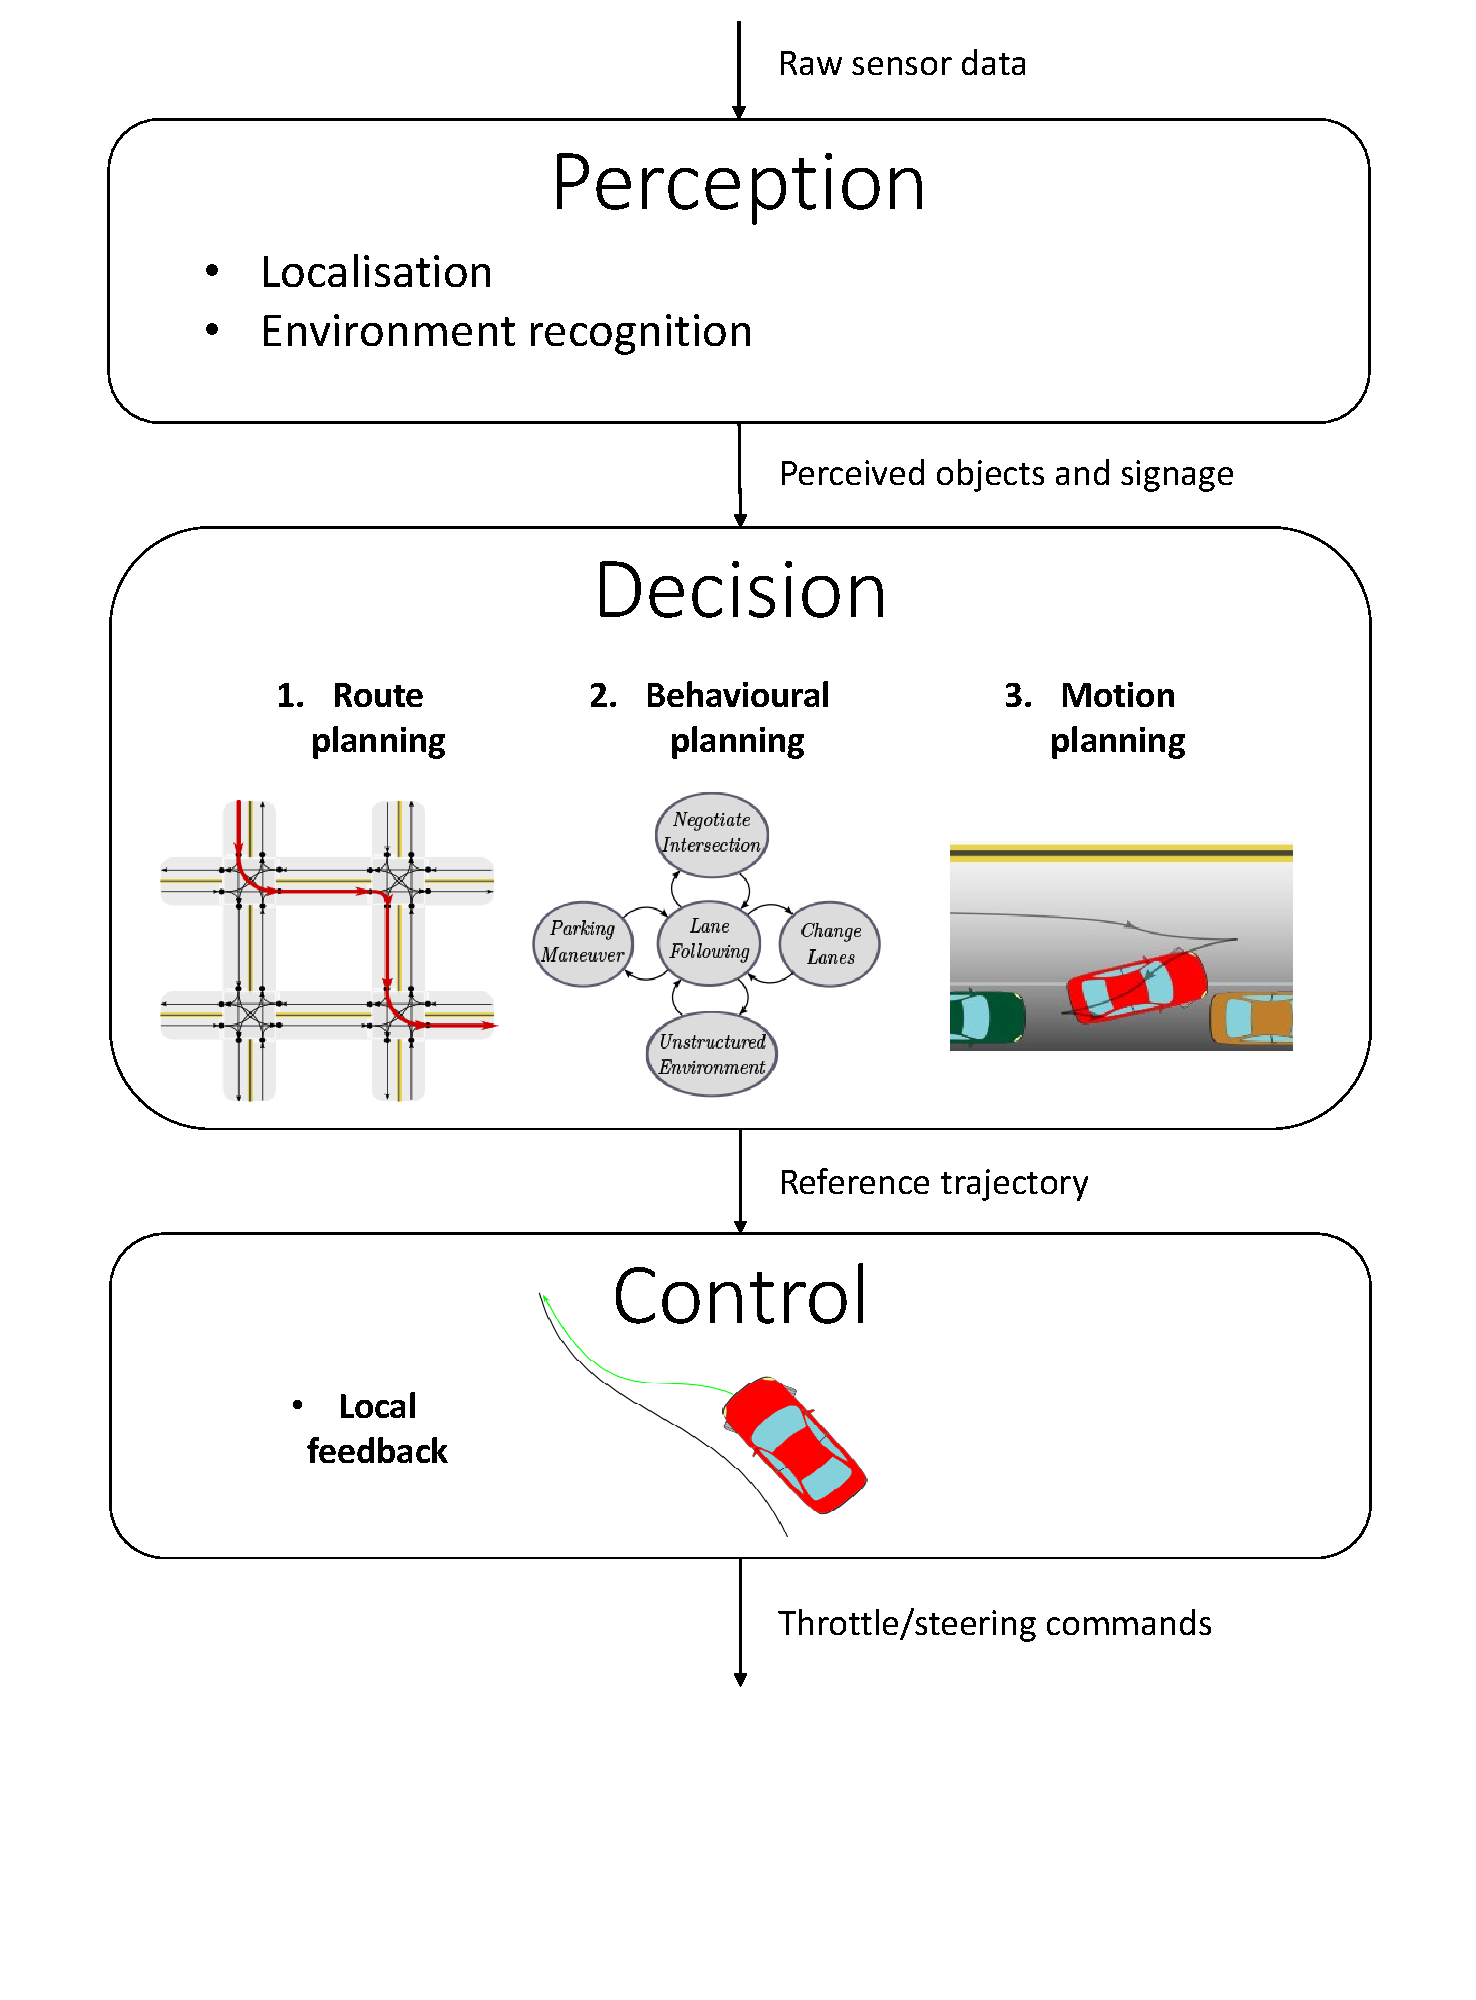
\includegraphics[trim={0 5cm 0 0}, clip, width=0.8\linewidth]{img/pipeline}
	\caption{The architecture of a typical self-driving software}
	\label{fig:robotics-pipeline}
\end{figure}

The traditional robotics pipeline, shown in \Cref{fig:robotics-pipeline}, involves three main modules: \emph{Perception}, \emph{Decision}, and \emph{Control} (also named Navigation, Guidance and Control in aerospace engineering). The \emph{Perception} module takes raw sensor data as input and produces a high-level reconstruction of the scene. Then, the \emph{Decision} module determines the desired trajectory of the vehicle. In the context of Autonomous Driving, a hierarchical structure is often used, with layers working at different timescales: first, a \emph{Route Planning} module queries a road network to find a global sequence of roads and intersections to take to reach the destination. Second, the \emph{Behavioural Layer} is responsible for considering real-time information to produce short-term goals and semantic decisions such as changing lane, yielding to a vehicle, etc. Third, \emph{Motion Planning} is responsible for generating a continuous feasible trajectory that implements the desired behaviour. Finally, the \emph{Control} module manipulates forces, by way of steering and throttle controls, to track the desired trajectory. Great research efforts have been made to resolve the two end-of-pipe tasks: Perception has benefited from the substantial progress in the field of Computer Vision due to the recent advent of Deep Learning. Many control schemes have been developed for ground vehicles to precisely follow a predefined trajectory, and are surveyed in \citep{Polack2018}.
In the Decision task, Route Planning is virtually solved and already provided by services such as \href{https://wiki.openstreetmap.org/wiki/Routing}{Open Street Maps}, and Motion Planning is well developed, as will be presented in \Cref{sec:sequential-decision-making}. However, we argue that Behavioural planning has been a neglected area: hitherto, most applications and challenges focused on simple settings with little complexity. In the DARPA Urban Challenge, all challengers reportedly used finite state machines for behavioural planning, whose transitions were triggered by handcrafted metrics based on velocity, proximity, and waiting zones \citep{Buehler2009}. 
In the industry, ADAS features such as LKA, ACC focus on highway driving with limited interaction. 


\paragraph{Decision-making under uncertainty}

Assume we have magically access to magical perception. Would we have solved the problem?
We still need to decide of how to act. Even if the present were known, the future would still be uncertain, because we do not know how other agents are going to act.
Human driving behaviour is not deterministic, but it is predictable. Highly structured.
Recall aletoric vs epistemic uncertainty?

Our objectives: 
1. Socially aware decision-making (account for other agents, and how our actions impact their behaviours)
2. A notion of safety. Risk as a constraint ? As a worst-case outcome?

\section{Contributions}

\paragraph{List of publications}